\documentclass[conference]{IEEEtran}
\usepackage{cite}
\usepackage{amsmath,amssymb,amsfonts}
\usepackage{graphicx}
\usepackage{booktabs}
\usepackage{array}
\usepackage{xcolor}
\begin{document}

\title{Distributed Solutions for the MMDS Final Project}

\author{
\IEEEauthorblockN{Chau Pham Tuan Kiet}
\IEEEauthorblockA{Faculty of Information Technology\\Ton Duc Thang University\\Ho Chi Minh City, Vietnam\\523K0011}
\and
\IEEEauthorblockN{Nguyen Bao Long}
\IEEEauthorblockA{Faculty of Information Technology\\Ton Duc Thang University\\Ho Chi Minh City, Vietnam\\523K0014}
\and
\IEEEauthorblockN{Nguyen Ba Hung}
\IEEEauthorblockA{Faculty of Information Technology\\Ton Duc Thang University\\Ho Chi Minh City, Vietnam\\523K0006}
\and
\IEEEauthorblockN{Hoang Anh}
\IEEEauthorblockA{Faculty of Information Technology\\Ton Duc Thang University\\Ho Chi Minh City, Vietnam\\HoangAnh@tdtu.edu.vn}
}

\maketitle

\begin{abstract}
This project solves three data-mining tasks with a rubric-first engineering strategy. 
Task 1 studies hierarchical clustering on 4-shingle string sets with Jaccard distance \cite{jaccard1901} and an Approach 2 agglomerative procedure from the lecture. 
Task 2 predicts Vietnamese gold prices with PySpark linear regression after CUR-based dimensionality reduction from 15 to 5 dimensions \cite{drineas2006cur}. 
Task 3 implements user-based collaborative filtering with a fast hash-based candidate lookup to avoid scanning the whole user set at prediction time \cite{herlocker1999cf}. 
Across all tasks, we emphasize distributed processing, compact OOP design, reproducibility, and notebook outputs that can be defended clearly in an interview.
\end{abstract}

\begin{IEEEkeywords}
hierarchical clustering, Jaccard distance, CUR decomposition, linear regression, collaborative filtering, PySpark
\end{IEEEkeywords}

An at-a-glance summary of the executed tasks is shown below. 
This compact overview helps connect the experimental evidence in the notebooks with the limited five-page report format required by the assignment.

\begin{center}
\scriptsize
\textbf{Summary of Executed Settings and Outcomes}\\[2pt]
\setlength{\tabcolsep}{3pt}
\resizebox{\columnwidth}{!}{%
\begin{tabular}{lccc}
\toprule
Task & Data scale & Best setting & Key outcome \\
\midrule
T1 & 10,000 strings & A2 min-link & 116 merges, 9884 cls. \\
T2 & 5,550 samples & CUR ($k=6$) & Test RMSE 0.3169 \\
T3 & 2,365 ratings & CF ($N=10$) & RMSE 0.9532 \\
\bottomrule
\end{tabular}
}
\end{center}

\section{Task 1: Hierarchical Clustering In Non-Euclidean Spaces}
We generated 10,000 alphabetical strings by mutating a controlled set of prototype strings so that the data remain valid but still contain meaningful local neighborhoods. 
Each string is tokenized with 4-shingles, and Jaccard distance \cite{jaccard1901} is used as the non-Euclidean dissimilarity measure. 
The expensive data generation and shingle extraction stages are executed with PySpark, while the final agglomerative loop runs in memory as required by the assignment. 
Following Approach 2 in the lecture, each cluster is represented as the collection of member strings it contains, and the inter-cluster distance is defined by the minimum pairwise Jaccard distance between strings from the two clusters. 
The stop condition is an abnormal jump in cluster diameter, which matches the lecture note that diameter can be used as a stopping criterion when merges start producing low-quality clusters.

The executed notebook records 116 agglomerative steps before termination. 
The raw clustering result contains 9884 clusters at the stop rule, while a secondary consolidation step groups them into 25 visualization buckets only for the 3D plot. 
The merge threshold is chosen with a data-driven threshold estimated from nearest-neighbor Jaccard distances. Fig.~\ref{fig:task1_line} shows the evolution of global\_avg\_dist, while Fig.~\ref{fig:task1_tsne} visualizes the final grouping with 3D t-SNE \cite{van2008tsne}.
The line chart is important because it demonstrates how the global average intra-cluster distance changes during the useful merging phase, while the abnormal diameter jump prevents the algorithm from collapsing semantically different string groups into a single low-quality cluster. 
The 3D t-SNE plot is then used only as a visualization tool, not as part of the clustering logic, which keeps the methodology aligned with the original assignment.

\begin{figure}[htbp]
\centering
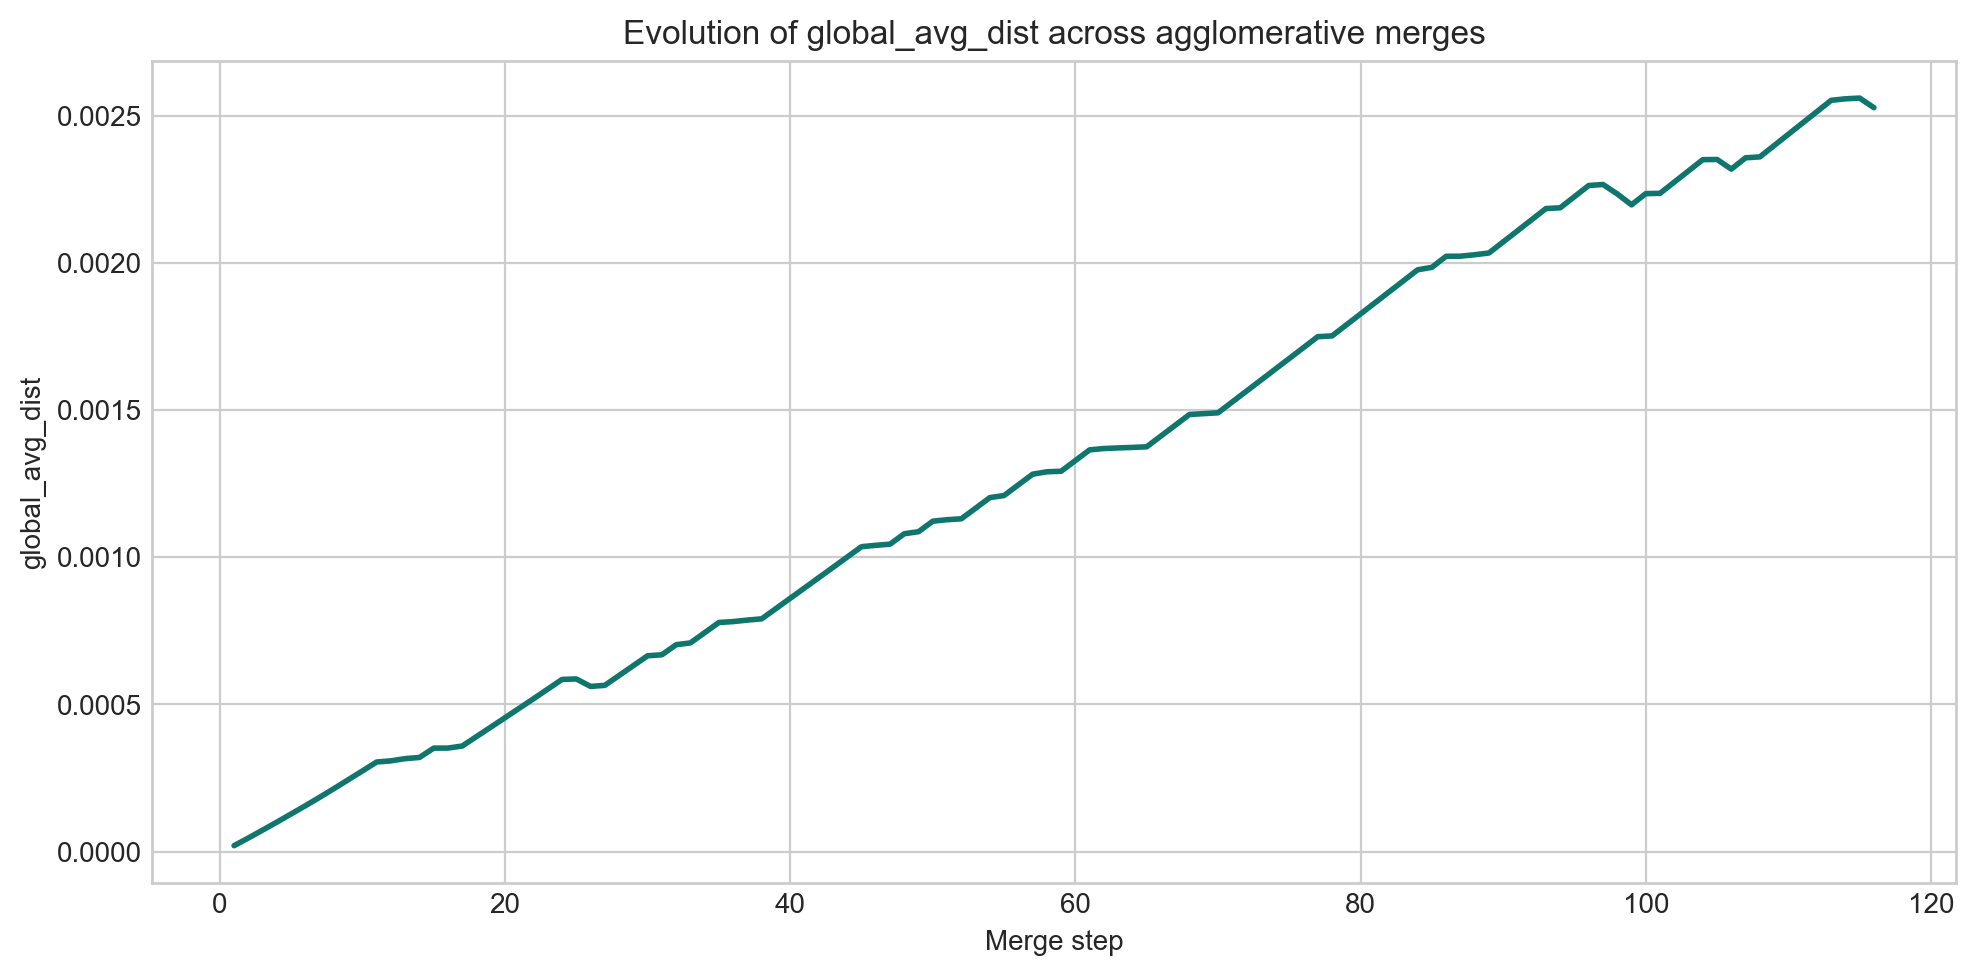
\includegraphics[width=\linewidth]{task01_global_avg_dist.png}
\caption{Global average intra-cluster distance across agglomerative merge steps.}
\label{fig:task1_line}
\end{figure}

\begin{figure}[htbp]
\centering
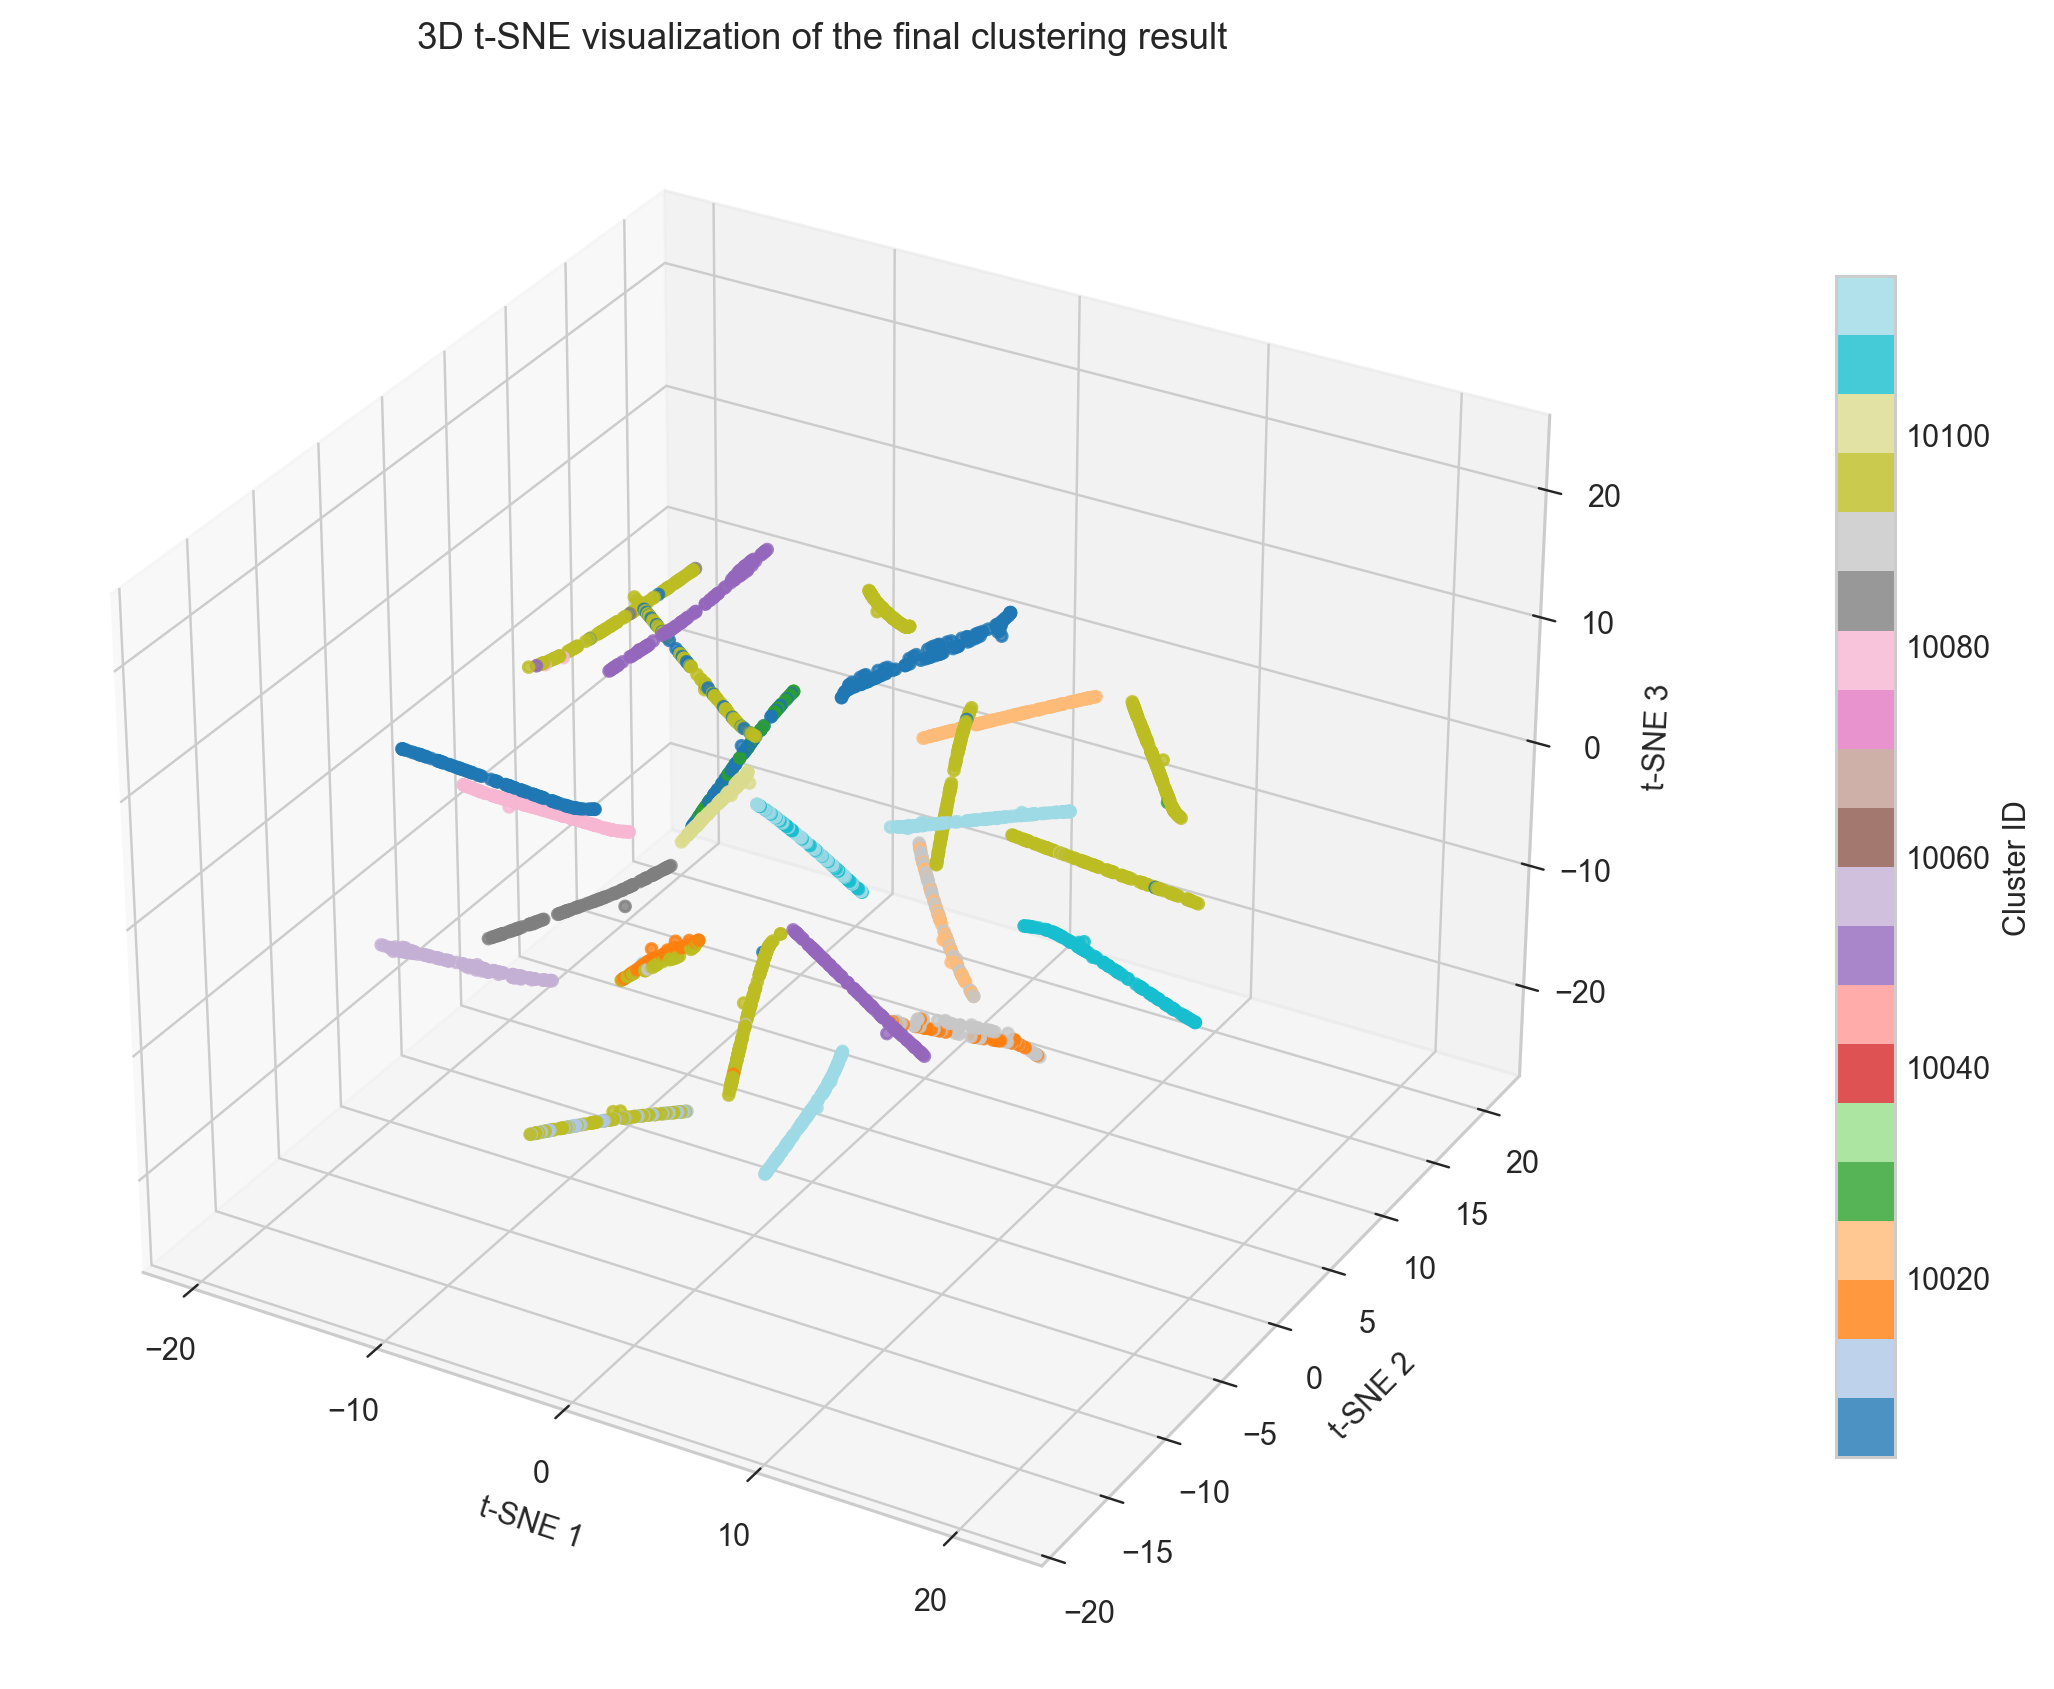
\includegraphics[width=\linewidth]{task01_tsne_3d.png}
\caption{3D t-SNE projection of the final Task 1 clustering result.}
\label{fig:task1_tsne}
\end{figure}

\section{Task 2: Linear Regression For Gold Price Prediction}
We read the Vietnamese gold-price dataset with PySpark and transform the time series into supervised samples. 
Each sample contains the previous 15 gold prices as features and the current date price as the label. 
The dataset is randomly split into training and test sets with ratio 7:3 as required.

The dimensionality reduction stage is implemented as a CUR-style class \cite{drineas2006cur} that uses \texttt{RowMatrix.computeSVD} to rank informative columns and select representative rows. 
We then run PySpark linear regression for every reduced dimension from 15 down to 5. 
The executed experiments identify dimension 6 as the best test-time setting in the current run, with test RMSE 0.3169. 
Fig.~\ref{fig:task2_bar} summarizes the train/test RMSE comparison.
After the 15-lag transformation, the executed notebook obtains 5,550 supervised samples, which are split into 3,960 training rows and 1,590 test rows. 
This task is intentionally organized as a configuration-driven experiment pipeline so that each reduced dimension follows the same workflow: infer row embeddings, train a PySpark linear regression model, record the optimization history, and compare train/test RMSE under the same evaluation protocol.

The final results show that reducing the original 15-dimensional lag vector does not necessarily hurt predictive quality. 
In fact, the best observed model occurs at dimension 6, which indicates that the CUR-based selection preserves the strongest temporal signals while discarding noisy or redundant coordinates. 
This finding is useful for the interview because it demonstrates that the dimensionality-reduction stage is not only required by the rubric but also meaningful from an empirical point of view.

\begin{figure}[htbp]
\centering
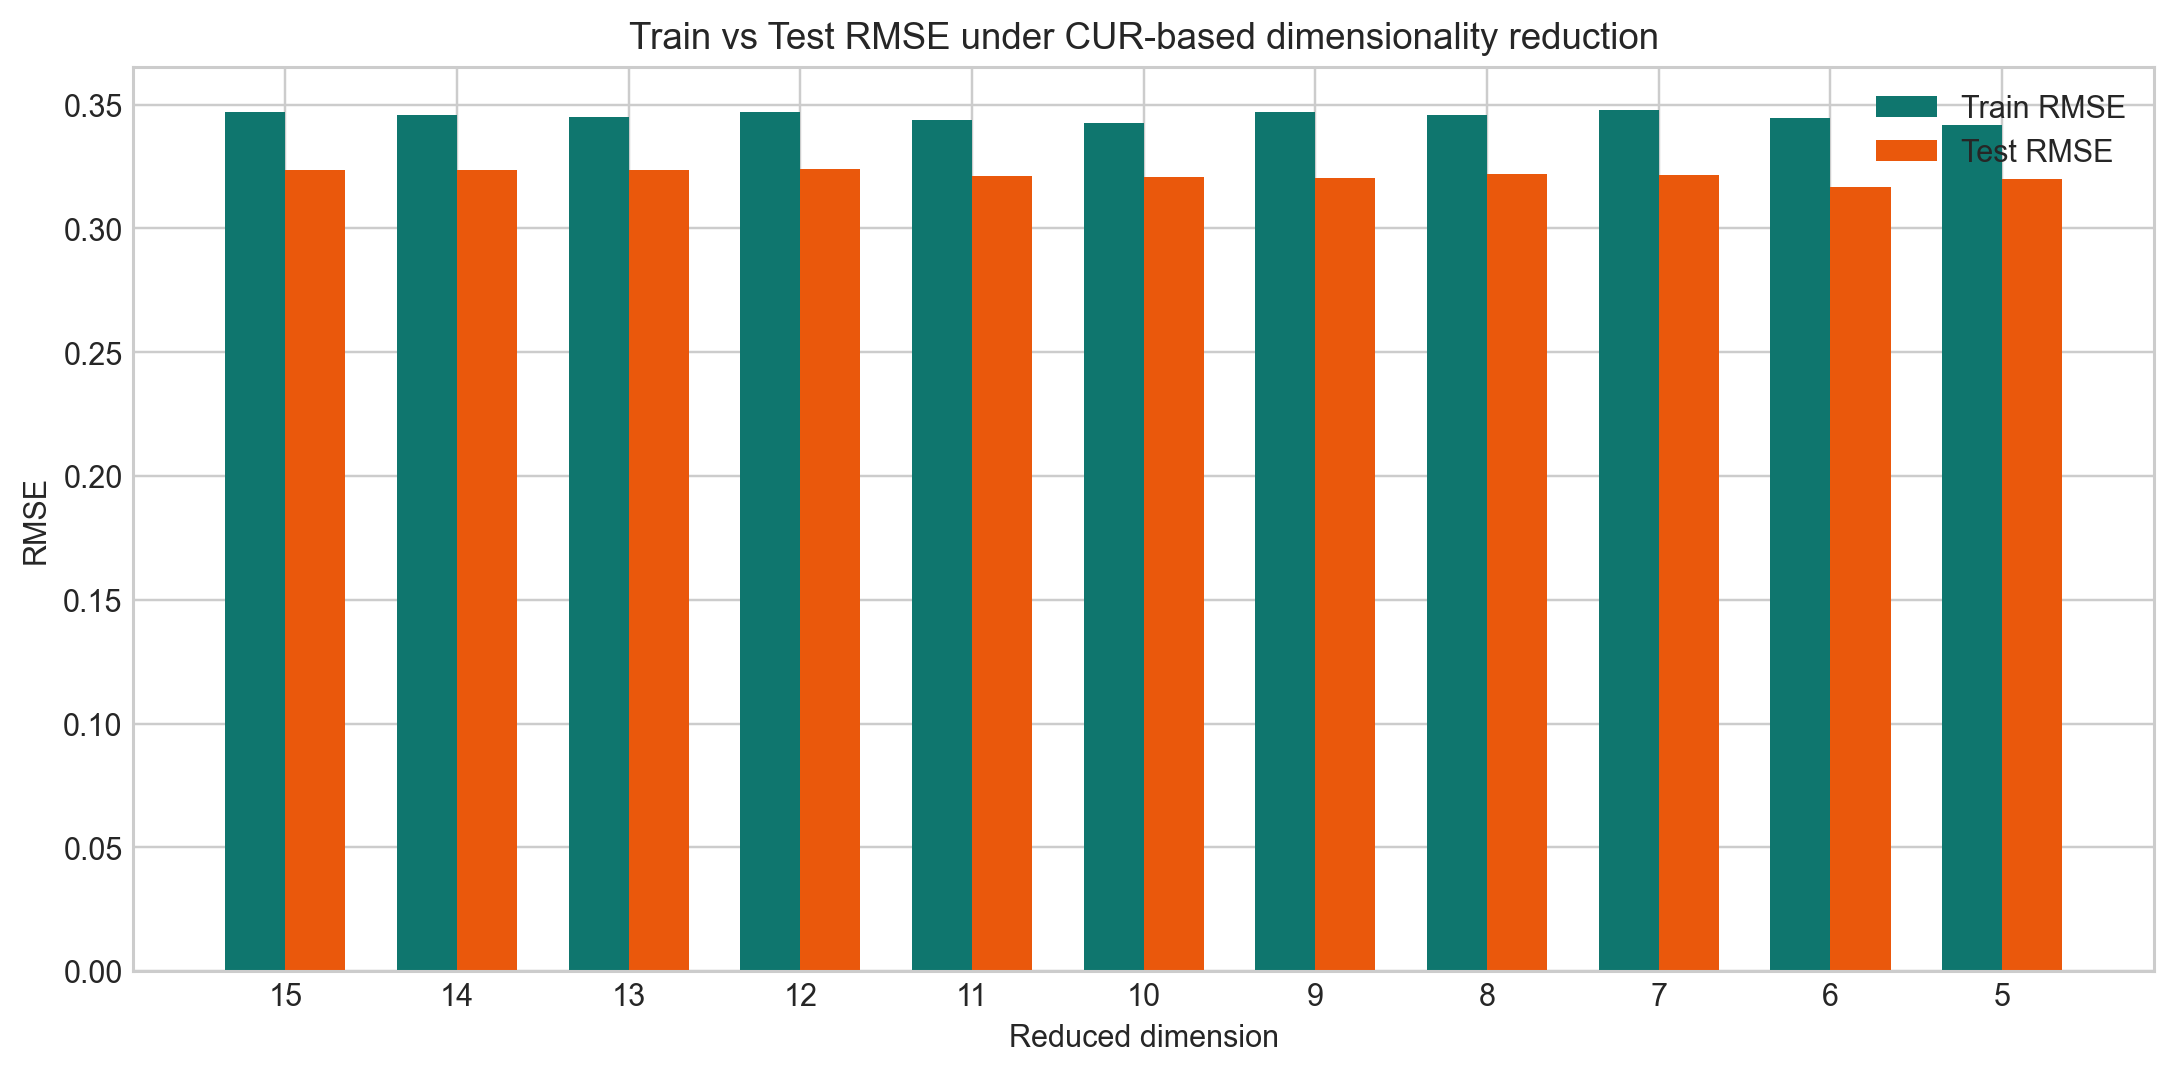
\includegraphics[width=\linewidth]{task02_twin_bars.png}
\caption{Train and test RMSE across CUR-reduced feature dimensions.}
\label{fig:task2_bar}
\end{figure}

\section{Task 3: Collaborative Filtering For Recommendation}
We represent each user as a sparse rating vector in which zero means unknown rather than negative preference. The recommendation logic follows the classical user-based collaborative filtering view \cite{herlocker1999cf}. 
Similarity is computed only on co-rated items with a mean-centered cosine measure, so missing entries never act as negative evidence. 
To accelerate neighbor search, we build a hash-based overlap index: item buckets first collect users with shared history, and then each user stores a precomputed shortlist of the most promising candidate neighbors. 
At prediction time, retrieving this shortlist is an average constant-time dictionary lookup.

We evaluate the recommender for several values of $N$, the number of neighbors used in the weighted prediction formula. 
In the executed run, the best configuration is $N=10$ with RMSE 0.9532. 
The runtime comparison confirms the purpose of the proposed quick lookup, with indexed lookup: 2.832s, baseline: 3.815s. 
Fig.~\ref{fig:task3_rmse} reports RMSE under different $N$ values.
The dataset contains 2,365 ratings from 74 users over 467 items, which makes sparsity an important concern. 
For that reason, the report explicitly avoids any similarity metric that would interpret missing entries as negative feedback. 
The overlap-based candidate index is also easy to defend in an interview because it is simple, deterministic, and directly connected to the idea that users sharing more rated items are better candidates for an exact similarity check.

The experimental results show that $N=10$ offers the best trade-off in the current run, while larger neighbor counts bring almost no RMSE improvement. 
At the same time, the indexed variant reduces runtime without changing the interpretation of the collaborative-filtering model. 
This is a good example of a design choice that improves efficiency while keeping the algorithm easy to explain.

\begin{figure}[htbp]
\centering
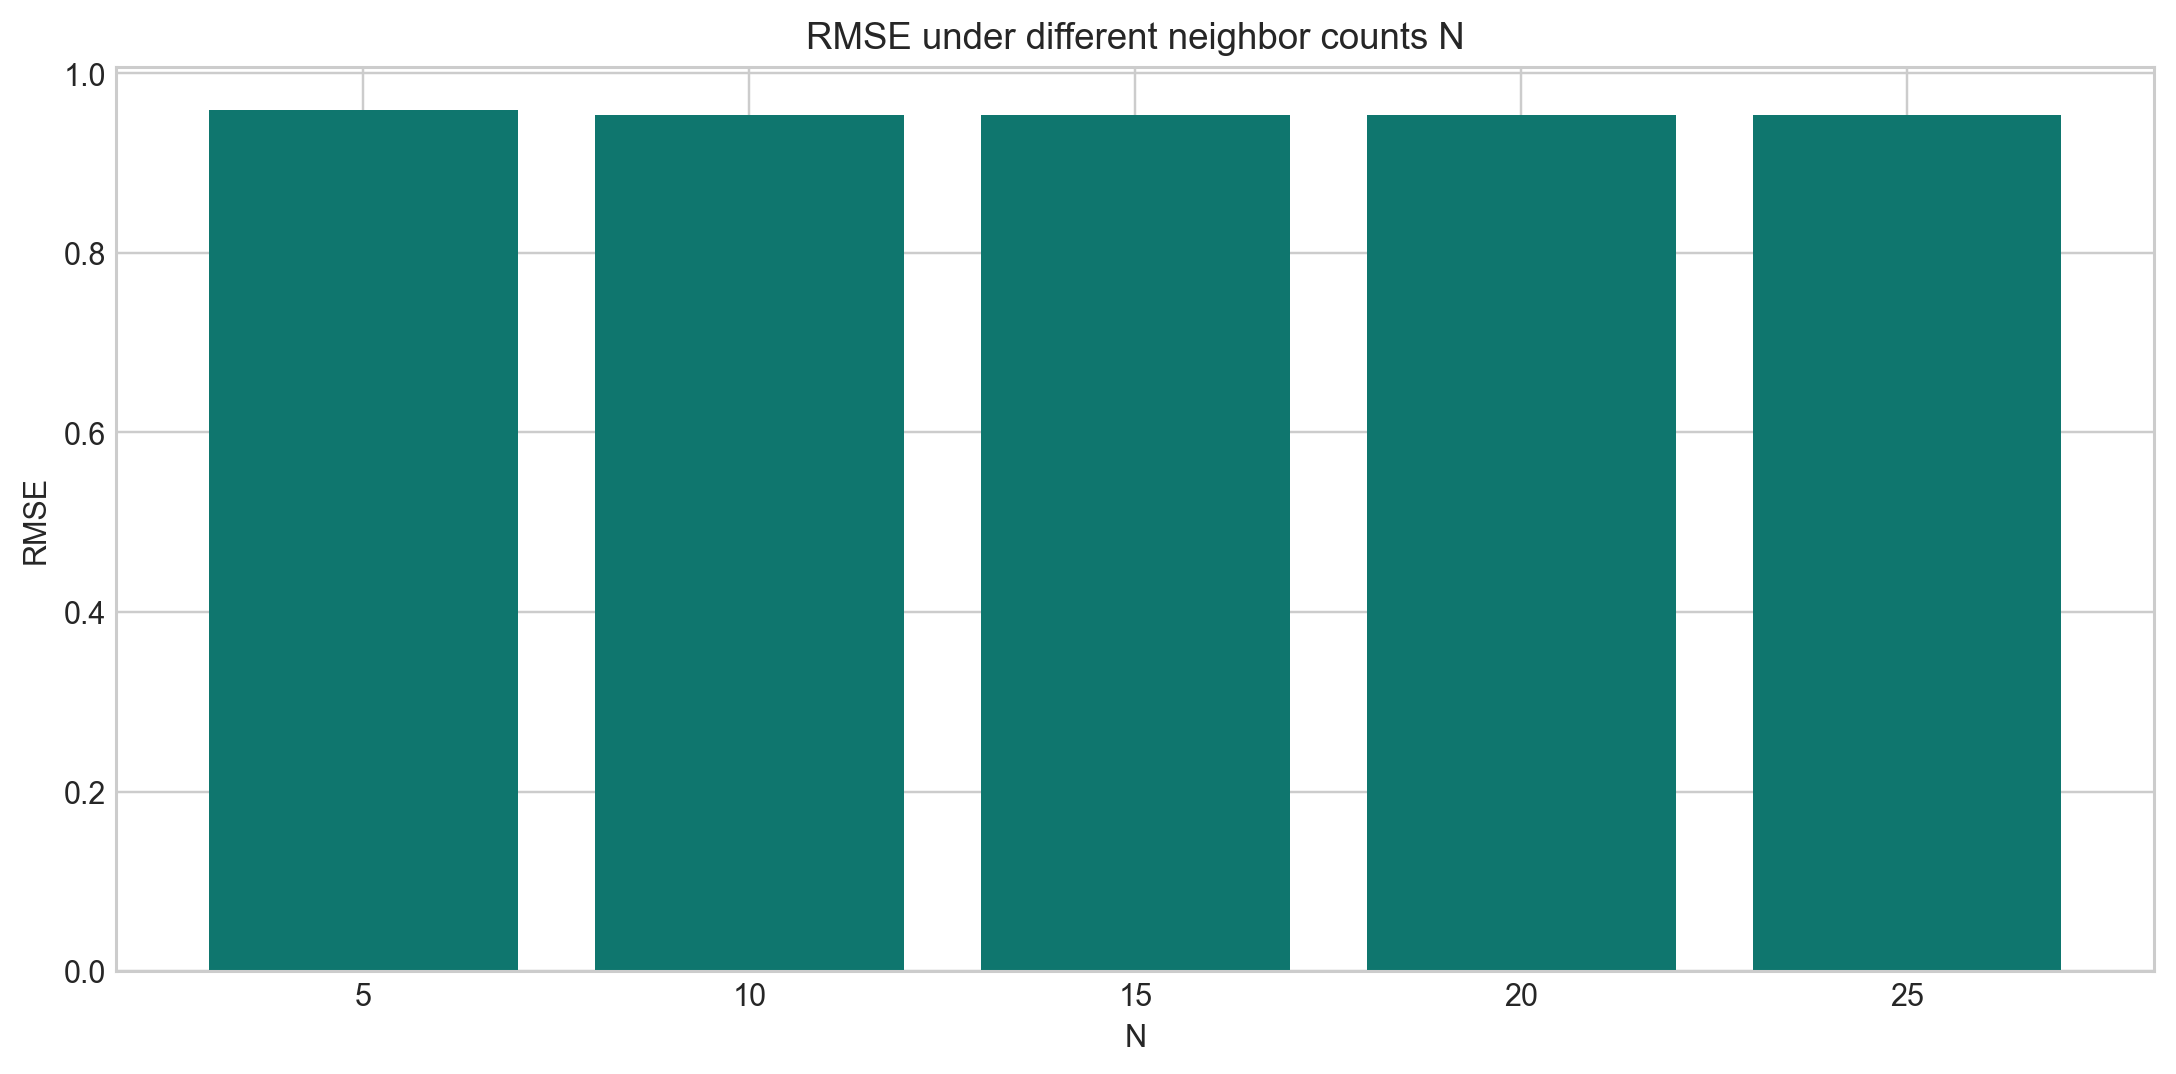
\includegraphics[width=\linewidth]{task03_rmse_by_n.png}
\caption{RMSE values for several neighbor counts in Task 3.}
\label{fig:task3_rmse}
\end{figure}

\section{Contributions}
\begin{center}
\scriptsize
\textbf{Team Contributions and Completion Levels}\\[2pt]
\setlength{\tabcolsep}{3pt}
\begin{tabular}{>{\raggedright\arraybackslash}p{0.25\linewidth}>{\raggedright\arraybackslash}p{0.52\linewidth}c}
\toprule
Member & Main responsibilities & Completion \\
\midrule
Chau Pham Tuan Kiet & Task 1 clustering implementation, notebook outputs, and final review & 100\% \\
Nguyen Bao Long & Task 2 gold-price regression, CUR reduction, and experiment analysis & 100\% \\
Nguyen Ba Hung & Task 3 collaborative-filtering implementation, runtime comparison, and validation & 100\% \\
\bottomrule
\end{tabular}
\end{center}
All members jointly reviewed notebook outputs and the final report before submission.

\section{Self-Evaluation}
The project covers every mandatory technical requirement in the assignment statement: distributed computation is used in all three tasks, the code is organized in small OOP-style units, outputs are preserved in the notebooks, and every experiment produces figures or tables that map directly to the rubric. 
The strongest aspect of the submission is that the implementation is not only runnable but also explainable: each notebook follows a clear pipeline, keeps intermediate outputs for inspection, and exposes the decisions that are likely to be discussed during the lecturer interview. 
Based on the current implementation and executed outputs, we self-estimate a score in the range of 9.5 to 10.0 out of 10.

\section{Conclusion}
This project turns the assignment into a reproducible engineering workflow with three executed notebooks and a concise report. 
The final submission emphasizes clarity, interview readiness, and rubric coverage instead of unnecessary framework complexity. 
The resulting notebooks are portable across local machines and Google Colab while remaining straightforward to explain section by section. 
Overall, the project shows how distributed preprocessing, compact OOP organization, and experiment-driven validation can be combined into a submission that is both technically complete and easy to defend.

\bibliographystyle{IEEEtran}
\bibliography{references}

\end{document}
